\documentclass{article}
\setcounter{secnumdepth}{-1}
\usepackage{graphicx}
\usepackage{amsfonts}
\usepackage{amsmath}
\usepackage{cite}
\usepackage[margin=0.9in, paperwidth=8.5in, paperheight=11in]{geometry}
\begin{document}
\title{S.I.E.V.E. Progress Report}
\author{Wayne Yang \\ Nick Kullman \\ Graham Clenaghan}
\date{Spring 2015}
\maketitle

\section{Sieve Analysis for Vaccine Trials}


\section{Sequence Data Visualization Tools}

There are several existing tools for the visualization of genomic / proteomic sequence data.  Some of these tools tend to provide a very detailed display of the alignments of sequences for a particular gene / protein from multiple patients.  While this approach allows a user to see all of their data at once, it does not provide quick and easy analysis of particular sites in the sequence across patients or subsets of patients.  The following example is from a software called Aliview \cite{aliview}.

\begin{center}
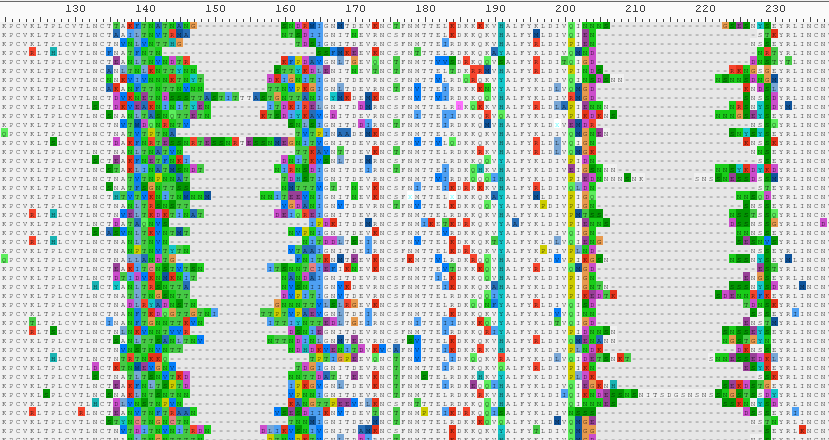
\includegraphics[height=3in,width=4in]{aliview.png}
\end{center}
Clearly, understanding the pattern of mutations and any relationships to treatment status for a particular site in the sequence is very difficult to do in this view with any precision.
\\
\newline
\noindent Other tools are geared towards specific analyses of sequence data.  The following figure was generated using WebLogo \cite{weblogo}, which is an online tool that can be used to parse sequence data and generate plots:
\begin{center}
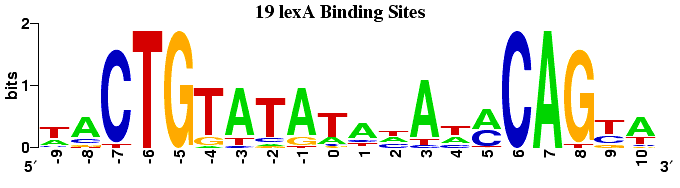
\includegraphics[height=1in,width=4in]{lexA.png}
\end{center}
Ignoring some of the aesthetic choices, the main issue is that the primary user interface looks like this:
\begin{center}
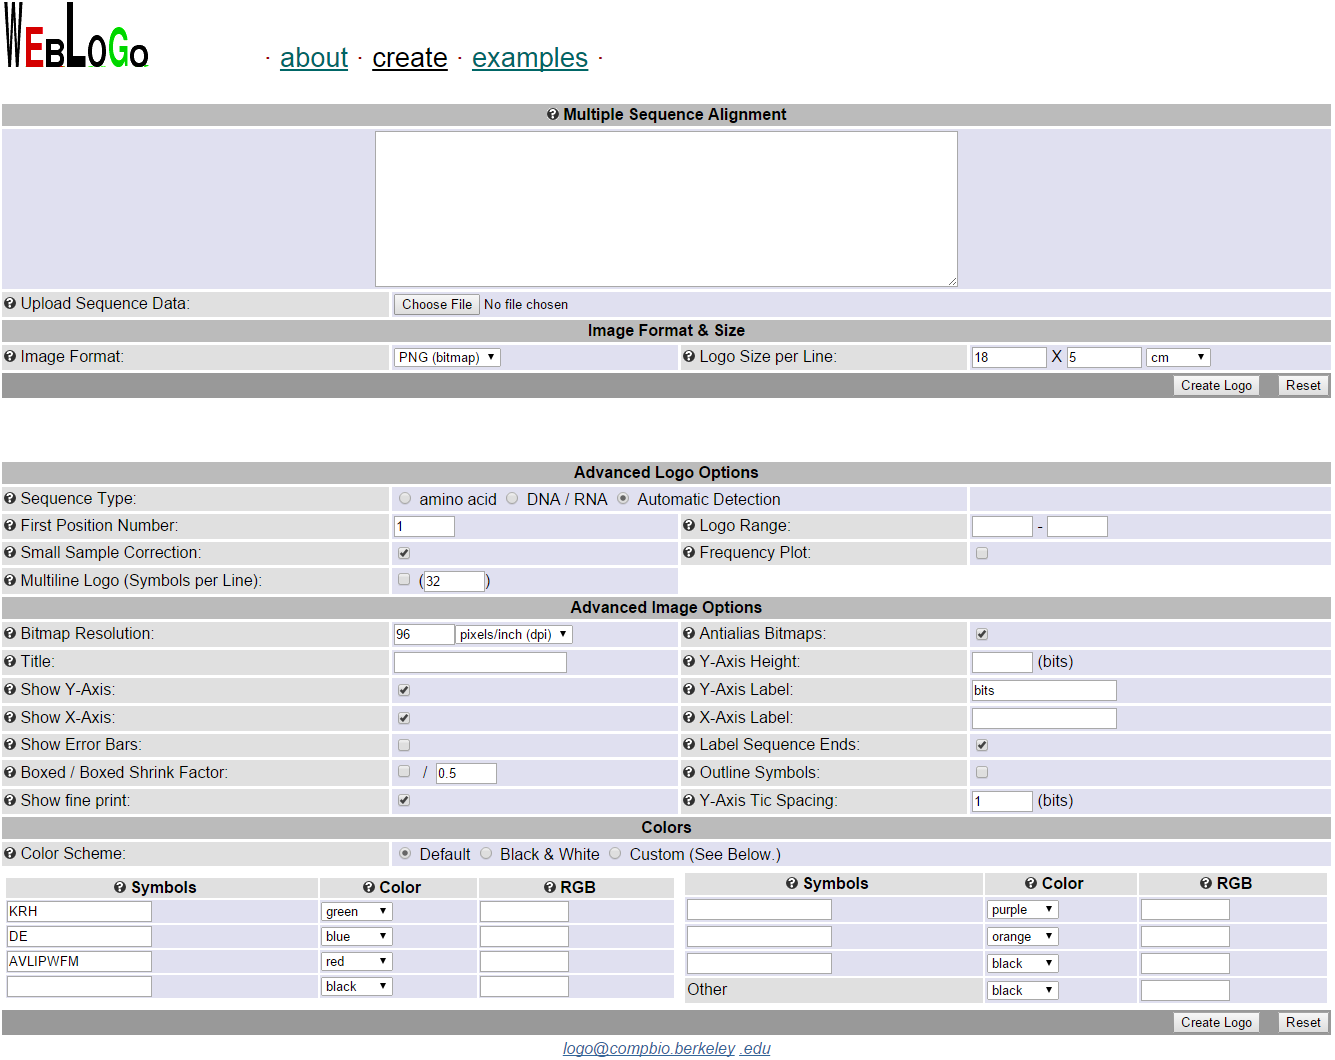
\includegraphics[height=3in,width=4in]{webloginterface.png}
\end{center}
While a graphic can be automatically generated, the user has to be quite specific about what is actually plotted.  As a result, if there are some sites that are known to be interesting, then a researcher can use WebLogo to construct plots.  However, this system makes exploratory data analysis and actually browsing the visualization rather difficult.
\\
\newline
\noindent Another tool that came up in our discussions with Dr. Gartland is the HIV Genome Browser, which allows users to browse reference data hosted online \cite{hivgenomebrowser}.   The browser is highly interactive and allows a user to explore the available sequences.   However, this visualization does not easily allow a user to import their own data and compare across patients and treatment groups as required by sieve analysis.  


\section{Project Plan}

The remaining tasks are roughly:
\begin{itemize}
\item Finalize the site selection mechanism / interface.  Primary member: Nick.
\item Color palette selection menu.  Primary member: Graham.
\item Incorporate p-values / entropy calculations. Wayne
\item Enable exporting of graphics. 
\item General polish / optimizations. 
\end{itemize}

\bibliographystyle{unsrt}
\bibliography{progress}

\end{document}

http://www.ncbi.nlm.nih.gov/pubmed/25095880

